\documentclass[../jarvis.tex]{subfiles}
\graphicspath{{\subfix{../images/}}}

\begin{document}
Complex numbers are just as complex as the name suggests, but they are so so elegant when used properly - from circles to trigonometric expressions, complex numbers link them all.
\begin{figure}[H]
    \centering
    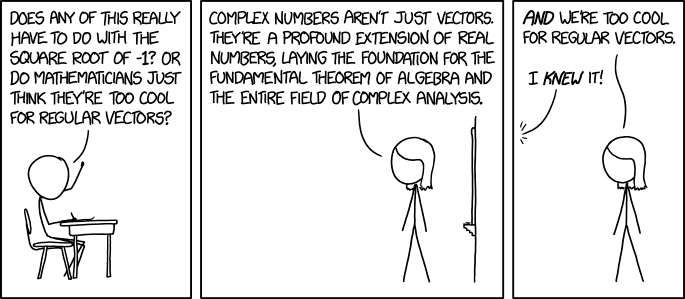
\includegraphics[scale=0.5]{xkcd_complex_numbers.png}
    \caption{Comic from https://xkcd.wtf/2028/}
\end{figure}

\subsection{Properties of Complex Numbers \ez}
Complex numbers can be written in a few ways, and each of these ways have their own benefits that make information more apparent.

\begin{proposition}[Notations for Complex Numbers]
    Let $z$ be a complex number and let $i$ be the imaginary number such that $i^2=-1$. We write $z=a+bi$ for real $a$ and $b$. 
    \begin{enumerate}    
    \item The \textit{real part} of $z$ is denoted as $Re(z)$ or $\Re(z)$. For instance, $\Re(z)=a$.
    \item The \textit{imaginary part} of $z$ is denoted as $Im(z)$ or $\Im(z)$. For instance, $\Im(z)=b$.
    \item The \textit{modulus} of $z$ is denoted as $|z|$. For instance, $|z|=\sqrt{a^2+b^2}$.
    \item The \textit{argument} of $z$ is denoted as $\arg z$. For instance, $\arg z=\tan^{-1} \left(\frac{b}{a}\right)$.
    \item The \textit{polar form} of $z$ can be written as
    $$z=re^{i\theta}=r(\cos\theta+i\sin\theta)=r\cis\theta.$$ Then, $|z|=r$ and $\arg z=\theta$.
    \item The \textit{conjugate} of $z$ is denoted as $\bar{z}$ or $z^*$. For instance, $$\bar{z}=a-bi=re^{-i\theta}=r(\cos\theta-i\sin\theta).$$
    \end{enumerate}
\end{proposition}
\begin{remark}
    Note that conjugation is distributive. For instance,
    \begin{enumerate}
        \item $\ol{z\pm w}=\ol{z}\pm\ol{w}$,
        \item $\ol{z\cdot w}=\ol{z}\cdot\ol{w}$,
        \item $\ol{\frac{z}{w}}=\frac{\ol{z}}{\ol{w}}$.
    \end{enumerate}
\end{remark}
With the different representations for complex numbers in mind, we shall briefly introduce some properties that relate to each form. As again, let $$z=a+bi=re^{i\theta}=r(\cos\theta+i\sin\theta).$$
\begin{proposition}[Absolute Square]
    $z\cdot\ol{z}=|z|^2$.
\end{proposition}
\begin{proof}
    \begin{align*}
        z\cdot\ol{z}&=(a+bi)(a-bi)=a^2-(bi)^2 \\
        &=a^2+b^2=(\sqrt{a^2+b^2})^2 \\
        &=|z|^2.
    \end{align*}
\end{proof}
\begin{proposition}[Rotation]
    Multiplying a complex number by $e^{i\theta}$ rotates the vector by $\theta$ radians counterclockwise about the origin.
\end{proposition}
\subsection{Exercise}
\problem Prove that $\arg(zw)=\arg(z)+\arg(w)$ and $\arg\left(\frac{z}{w}\right)=\arg(z)-\arg(w)$.
\problem De Moivre's theorem states that $$\left(\cos\theta+i\sin\theta\right)^n=(\cos n\theta+i\sin n\theta).$$ Prove de Moivre's theorem by induction.

\subsection{Roots of Unity \med}
Let $n$ be a positive integer. An $n$th \textit{root of unity} is a complex number $z$ that satisfies the equation $$z^n=1.$$

Then, the $n$th roots of unity can be described by 
$$z=\exp\left(\frac{2k\pi}{n}\right)=\cos\frac{2k\pi}{n}+i\sin\frac{2k\pi}{n},\quad k=0,1,\cdots,n-1.$$

\begin{proposition}[Conjugates]
    If $z$ satisfies $z^n=1$, meaning $z$ is an $n$th root of unity, then so does $\ol{z}$.
\end{proposition}
\begin{proof}
    Recall that $z\cdot\ol{z}=|z|^2=1,$ so $\ol{z}=\frac{1}{z}=z$.
\end{proof}

To start off the section, we showcase a trick on evaluating (suspiciously convenient) trigonometric sums through the lenses of the \textbf{roots of unity}.
\begin{example}[2021 H2 Further Math P1/9]
Let $\omega=\cos{\frac{2\pi}{11}}+\sin{\frac{2\pi}{11}}$.
Show that $$\sum_{j=1}^{10} \omega^{j}=-1.$$
\end{example}
Simple enough, $\omega$ is an 11th roots of unity, and so it satisfies the polynomial $z^{11}-1=0$. Moreover, the required sum is a geometric progression, so
$$\sum_{j=1}^{10} \omega^{j}=\frac{\omega^{11}-1}{\omega-1}-1=-1.$$

\begin{example}[cont.]
The complex numbers $\alpha$ and $\beta$ are such that
$$\alpha=w+w^3+w^4+w^5+w^9 \text{ and } \beta=w^{-1}+w^{-3}+w^{-4}+w^{-5}+w^{-9}.$$
Find in its simplest form, the quadratic equation whose roots are $\alpha$ and $\beta$.
\end{example}
Most jarringly, the exponents for $\alpha$ don't come in order: it jumps from 1 to 3, then 5 to 9 and $\beta$ mirrors this behaviour, except with negative exponents. Fortunately, we see that $w^9=e^{\frac{18\pi i}{11}}=e^{\frac{-4\pi i}{11}}=w^{-2}$ and that $\Re(w^{-2})=\Re(w^2)$ (why doesn't the problem use $w^2$ and $w^{-2}$ instead?). We also make a mental note that $\alpha=\beta^{*}$. Maybe this will come in handy later.

For now, we have
\begin{align*}
    \alpha+\beta &= (w+w^{-1})+(w^3+w^{-3})+(w^4+w^{-4})+(w^5+w^{-5})+(w^9+w^{-9}) \\
    &= 2\Re(w+w^3+w^4+w^5+w^9) = 2\Re(w+w^2+w^3+w^4+w^5) \\
    &= 2\left(\cos{\frac{2\pi}{11}}+\cos{\frac{4\pi}{11}}+\cos{\frac{6\pi}{11}}+\cos{\frac{8\pi}{11}}+\cos{\frac{10\pi}{11}}\right)
\end{align*}
This is usually a tough sum to evaluate, but the values here just line up way too nicely for us to ignore... With that, here comes the \textit{trick:}  $$S=\cos{\frac{2\pi}{11}}+\cos{\frac{4\pi}{11}}+\cos{\frac{6\pi}{11}}+\cos{\frac{8\pi}{11}}+\cos{\frac{10\pi}{11}}.$$ We consider
\begin{align*}
    \frac{S\cdot2\sin{\frac{2\pi}{11}}}{2\sin{\frac{2\pi}{11}}} &= \frac{2\sin{\frac{2\pi}{11}}\cos{\frac{2\pi}{11}}+2\sin{\frac{2\pi}{11}}\cos{\frac{4\pi}{11}}+\cdots +2\sin{\frac{2\pi}{11}}\cos{\frac{10\pi}{11}}}{2\sin{\frac{2\pi}{11}}}\\
    &= \frac{\sin{\frac{10\pi}{11}}+\sin{\frac{12\pi}{11}}-\sin{\frac{2\pi}{11}}}{2\sin{\frac{2\pi}{11}}} &&\text{using the product-to-sum formula}\\
    &= -\frac{1}{2}
\end{align*}
\begin{remark}
This doesn't work if we have one fewer term though. For instance if we exclude $\cos{\frac{10\pi}{11}}$, then the sum doesn't come out nice anymore. Hmm...
\end{remark}
Hence, $\alpha+\beta=-1$. Furthermore, we have $w^{-i}=w^{-11+i}$ and $w^i=w^{11-i}$, so that
\begin{align*}
    \alpha\beta&=(w+w^3+w^4+w^5+w^9)(w^{-1}+w^{-3}+w^{-4}+w^{-5}+w^{-9}) \\
    &=5+w^{-8}+w^{-6}+w^{-5}+2w^{-4}+w^{-3}+2w^{-2}+2w^{-1}+2w+2w^2+w^3+2w^4+w^5+w^6+w^8 \\
    &=5+(w^{-10}+w^{-9}+\cdots+w^{-1})+(w+w^2+\cdots+w^{10}) \\
    &=5+\sum_{j=1}^{10} \omega^{j}+\left(\sum_{j=1}^{10} \omega^{j}\right)^{*} = 3
\end{align*}
where the final sum holds because 
$$\left(\sum_{j=1}^{10} \omega^{j}\right)\left(\sum_{j=1}^{10} \omega^{j}\right)^{*}=\left|\left(\sum_{j=1}^{10} \omega^{j}\right)\right|^2=1$$
Hence, a possible quadratic equation is $x^2-x+3=0$.
\begin{example}[cont..]
Prove that $|\alpha|=\sqrt{3}$
\end{example}
Aha! Here's where the property that $\alpha=\beta^{*}$ comes in handy. 
$$|\alpha|^2=\alpha\cdot\alpha^{*}=\alpha\beta=3$$
and the result follows.

\begin{example}[cont...]
Prove that $$\sin{\frac{2\pi}{11}}+\sin{\frac{6\pi}{11}}+\sin{\frac{8\pi}{11}}+\sin{\frac{10\pi}{11}}+\sin{\frac{18\pi}{11}}=\frac{\sqrt{11}}{2}.$$
\end{example}
Observe that this is simply the imaginary part of $\alpha$. In addition, 
\begin{align*}
    \Im(\alpha)&=\sin{\frac{2\pi}{11}}+\sin{\frac{6\pi}{11}}+\sin{\frac{8\pi}{11}}+\sin{\frac{10\pi}{11}}+\sin{\frac{18\pi}{11}} \\
    &=\sin{\frac{2\pi}{11}}+\sin{\frac{6\pi}{11}}+\left(\sin{\frac{8\pi}{11}}-\sin{\frac{7\pi}{11}}\right)+\sin{\frac{10\pi}{11}} \\
    &> 0
\end{align*}
since each term is positive.
Thus, 
\begin{align*}
    \Im(\alpha)&=\frac{1}{2}\cdot2\Im(\alpha))=\frac{1}{2}\left(\alpha-\alpha^{*}\right)\\
    &=\frac{1}{2}\left(\alpha-\beta\right) \\
    &=\frac{1}{2}\Im\left(\sqrt{(\alpha+\beta)^2-4\alpha\beta}\right) \\
    &=\frac{\sqrt{11}}{2}
\end{align*}
by taking the positive square root because $\alpha-\beta=2\Im(\alpha)>0$.
\paragraph{Tangent: Gaussian Periods}
So why didn't the question use $w^{-2}$ and $w^2$? The set $(1,3,4,5,9)$ feels too specific anyways. As it turns out, this is the set of \textbf{quadratic residues} modulo 11 (prove this!), and the sums $\alpha$ and $\beta$ are the so-called quadratic Gauss sums:
\begin{definition}[Quadratic Gauss Sum]
$$g_a=\sum_{t=0}^{p-1}\left(\frac{t}{p}\right)\zeta^{at}$$
\end{definition}
where $\left(\frac{t}{p}\right)$ is the Legendre's symbol
\begin{definition}[Legendre's symbol]
$\left(\frac{t}{p}\right)=
\begin{cases}
$1$ &\text{if $t$ is a quadratic residue,}\\
$-1$ &\text{if $t$ is a quadratic non-residue,}\\
$0$ &\text{if $p|t$.}
\end{cases}$
\end{definition}
In what follows, we showcase a technique of \textit{summing in two ways} that reduces this problem to a sum of roots of unity.

\begin{proposition}[Expressing $g_a$ in terms of $g_1$]
$$g_a=\left(\frac{a}{p}\right)g_1.$$
\end{proposition}
\begin{proof}
Firstly if $p|a$, then $g_a=0$ (why?).

Henceforth, suppose $p$ does not divide $a$. Then,
$$\left(\frac{a}{p}\right)g_a=\sum_{t=0}^{p-1}\left(\frac{at}{p}\right)\zeta^{at}=\sum_{x=0}^{p-1}\left(\frac{x}{p}\right)\zeta^x=g_1.$$
The first equality follows because $a \nmid p \implies at \nmid p$, so that as $t$ runs over the set of residues (mod $p$), then so does $at$. Since $at$ runs over the set of residues, then we may simply let the sum run over all $x$ in the set of residues (mod $p$).

Now observe by definition that $\left(\frac{a}{p}\right)^2=1$, and we are done.
\end{proof}
What follows is the \textit{coup de grace}:
\begin{proposition}[Summing in two ways]
$$g_1^2=(-1)^{\frac{p-1}{2}}p.$$
\end{proposition}
For convenience, write $g=g_1$. According to Ireland-Rosen, the main idea is to consider the sum $\sum_{a=0}^{p-1}g_ag_{-a}$ in two ways. Again, we consider only the case when $p\nmid a$.

On one hand, we have $$g_ag_{-a}=\left(\frac{a}{p}\right)\left(\frac{-a}{p}\right)g^2=\left(\frac{-1}{p}\right)g^2,$$ whence it follows that
$$\sum_{a=1}^{p-1}g_ag_{-a}=\left(\frac{-1}{p}\right)(p-1)g^2.$$

On the other hand, we have
$$g_ag_{-a}=\sum_{x=0}^{p-1}\sum_{y=0}^{p-1}\left(\frac{x}{p}\right)\left(\frac{y}{p}\right)\zeta^{a(x-y)},$$
and summing both sides over $a$,
\begin{align*}
  \sum_{a=0}^{p-1}g_ag_{-a}&=\sum_{a=0}^{p-1}\sum_{x=0}^{p-1}\sum_{y=0}^{p-1}\left(\frac{x}{p}\right)\left(\frac{y}{p}\right)\zeta^{a(x-y)} \\
  &=\sum_{x=0}^{p-1}\sum_{y=0}^{p-1}\left(\frac{x}{p}\right)\left(\frac{y}{p}\right)\sum_{a=0}^{p-1}\zeta^{a(x-y)} \\
  &=\sum_{x=0}^{p-1}\sum_{y=0}^{p-1}\left(\frac{x}{p}\right)\left(\frac{y}{p}\right)s(x,y)p \\
  &= p(p-1)
\end{align*}
where we have $p^{-1}\sum_{t=0}^{p-1}\zeta^{at}=s(x,y)=\begin{cases}
$1$ &\text{if $p\mid t$} \\
$0$ &\text{otherwise}.
\end{cases}$.
Putting both parts together, the result follows.
\end{document}